% A poster using beamerposter and the gemini theme with epfl colors.
% Beamerposter will let you create a poster in a single beamer frame
% using the columns and blocks from the beamer class.
% The color theme is adapted from Gemini's MIT scheme.

% use beamer as documentclass
\documentclass[final]{beamer}

% use the beamerposter package to create a poster
\usepackage[scale=1.4,orientation=portrait,size=a0]{beamerposter}
\usepackage{csquotes}
\usepackage[backend=biber,firstinits=true,maxbibnames=99,bibencoding=utf8,style=numeric]{biblatex}
\addbibresource{references.bib}
% make references small
\renewcommand*{\bibfont}{\scriptsize}

% use the gemini theme. 
\usetheme{gemini}
% If you prefer heavier fonts (looks nicer on screen):
% \setbeamerfont{block body}{family=\Lato}
% use the epfl color theme, defining epfl{dark}red, -{dark}green,  -light, -gray, and -dark
\usecolortheme{epfl}

\usepackage{lyluatex}
\usepackage{booktabs}
\usepackage{amsmath}
\usepackage{graphicx}
\usepackage{tikz}
\usepackage{adjustbox}
\usepackage{qrcode}
\usepackage{wrapfig}
\usepackage{tikz-qtree}
\usepackage{pgfplots}
\pgfplotsset{compat=1.15}

% set OPG options
\tikzset{operation/.style={below,sloped,inner sep=1pt}} % with labels
% \tikzset{operation/.style={text opacity=0}} % without labels
\tikzset{external node/.style={}}
\tikzset{epsilon node/.style={}}
\tikzset{note node/.style={}}
\tikzset{every edge/.append style={line width=2.5pt}}
\tikzset{epsilon edge/.style={draw=epflgray}}
\tikzset{external edge/.style={draw=epflgray}}
% \tikzset{surface edge/.style={very thick}} % mark surface with thick edges
\tikzset{surface edge/.style={}} % don't mark surface

\newcommand{\generates}{\Rightarrow}
\newcommand{\dir}{\rightarrowtail}
\newcommand{\raga}{r\=aga}
\newcommand{\alap}{\=al\=ap}
\newcommand{\multani}{Mult\=an\=i}


\title{\Huge Ist das Kunst oder kann das weg? \\ \huge Analysen und ein Experiment zu KI-generierten Chorälen}
\author{Jason Ackermann, Ricarda Ernsperger, Adam Moeslein,\\ Angelina Tarlovskaia, Hendrik Weiß, \& Fabian C. Moss}
\institute{Institut für Musikforschung | Julius-Maximilians-Universität Würzburg}


\begin{document}

\begin{frame}[t]

  \vfill
  
  \begin{columns}[t]
    \begin{column}{0.25\textwidth}
      \begin{block}{Einführung}
        Im Wintersemester 2025/26 haben sich Studierende im Seminar 
        ``Themen der Digitalen Musikforschung'' unter anderem mit 
        Musik und Künstlicher Intelligenz auseinander gesetzt und dabei 
        insbesondere das Tool \alert{NotaGen}~\autocite{notagen} ausprobiert. 

        Nachdem mit einigem Aufwand NotaGen zum Laufen gebracht werden konnte,
        wurden verschiedene Stücke generiert. NotaGen akzeptiert Prompts in der Form:

        \texttt{<composer><epoch><instrumentation>}
        
        Daraufhin werden Dateien im \texttt{.musicxml}-Format generiert,
        die mit herkömmlichen Notationsprogrammen
        geöffnet und abgespielt werden können.

        % Melodies of \alap\ performances can be understood as the result of \alert{recursive elaboration}
        % of \alert{notes} and \alert{intervals}.
        %
        % \vspace{2em}
        %
        % \begin{tikzpicture}[overlay,font=\small]
        %   \node at (2.5,3.5) {step:};
        %   \node at (4.5,3.5) {1};
        %   \node at (8,3.5) {2};
        %   \node at (14,3.5) {3};
        % \end{tikzpicture}
        % 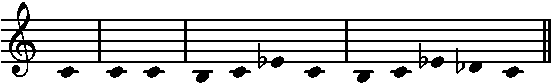
\includegraphics[width=\columnwidth]{figures/alap-phrase.pdf}
        % \begin{center}
        %   \begin{small}
        %     A melody derived in three steps.
        %   \end{small}
        % \end{center}
        %
        % \vspace{1em}
        %
        % Elaborations of notes include \alert{duplication} (1) and left or right \alert{neighbors} (2).
        % Interval elaborations include \alert{passing notes} (3) and \alert{linear fills}.
        
      \end{block}
    \end{column}

    \begin{column}{0.25\textwidth}
      \begin{block}{Qualitative Musikanalyse}
        Auf der Internetseite \url{https://electricalexis.github.io/notagen-demo/}
        bieten die Autoren von NotaGen verschiedene Beispiele an, an denen die 
        Fähigkeiten des Systems dargestellt werden sollen. 

        Bei den von uns gestellten Beispielen viel aber auf, dass 
        NotaGen häufig zu langen \alert{Wiederholungen} von Motiven neigt, 
        dass der \alert{Ambitus} von Instrumenten oder Stimmen nicht immer eingehalten wird, 
        und dass manchmal \alert{Vorzeichenfehler} vorkommen, die sich dann fortsetzen und zu stark 
        dissonanter Musik führen. 

           % A mode is a scale together with a \alert{hierarchy of stability}
        % among the scale degrees and restrictions on their \alert{movement direction}.
        %
        % \vspace{1em}
        %
        % 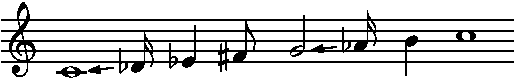
\includegraphics[width=\linewidth]{figures/scale.pdf}
        %
        % \begin{center}
        %   \begin{small}
        %     The tonal hiearchy of \raga\ \multani.
        %   \end{small}
        %
        %   \vspace{1.3em}
        %
        %   \setlength{\tabcolsep}{15pt}
        %   \begin{tabular}{lccccccc}
        %     \toprule
        %     pitch & 1 & \flat 2 & \flat 3 & \sharp 4 & 5 & \flat 6 & 7 \\
        %     \midrule
        %     direction & $\updownarrow$ & $\downarrow$ & $\updownarrow$ & $\updownarrow$
        %                                              & $\updownarrow$ & $\downarrow$ & $\updownarrow$\\ 
        %     stability & 4 & 0 & 2 & 1 & 3 & 0 & 2 \\
        %     \toprule
        %   \end{tabular}
        % \end{center}
        
        % Melodic elaboration respects both the hierarchical level and the directionality
        % of the scale degrees.
      \end{block}
    \end{column}

    \begin{column}{0.25\textwidth}
      \begin{block}{Empirische Überprüfung}
        Zur Validierung unserer qualitativen Analysen haben wir zwei Experimente durchgeführt:
        \begin{enumerate}
          \item Vergleichende \alert{statistische Analyse} von Bach-Chorälen mit von NotaGen generierten.
        (NB: Wir haben nur 100 NotaGen-Choräle generiert!)
      \item Ein \alert{Wahrnehmungsexperiment}, in dem Teilnehmende raten müssen, ob vorgespielte Choräle 
            von einem Menschen (Bach) oder einem Algorithmus (NotaGen) komponiert wurden. (NB: Aus praktischen 
            Gründen werden keine kompletten Kompositionen vorgespielt, sondern nur einzelne Phrasen.)
        \end{enumerate}
        %
        % Neighbors and passing notes can be \alert{non-adjacent}
        % if they respect the tonal hierarchy of the mode.
        %
        % \vspace{0.5em}
        %
        % \begin{center}
        %   \begin{tikzpicture}
        %     \begin{axis}[
        %       ybar=0pt,
        %       /pgf/bar shift=0pt,
        %       bar width=25pt,
        %       symbolic x coords={{$7_\prime$},$1$,$\flat 2$,$\flat 3$,$\sharp 4$,$5$,$\flat 6$,$7$,$1'$,$\flat 2'$},
        %       xtick={{$7_\prime$},$1$,$\flat 2$,$\flat 3$,$\sharp 4$,$5$,$\flat 6$,$7$,$1'$,$\flat 2'$},
        %       ymajorticks=false,
        %       % axis y line=none,
        %       axis x line*=bottom,
        %       axis line style={draw=none},
        %       tick style={draw=none},
        %       height=7cm, width=\linewidth,
        %       ymin=0, ymax=5,% ylabel={\small hierarchical level}
        %       ]
        %       \addplot [draw=none,fill=uva-rood] coordinates {
        %         ($\flat 3$,3)
        %       };
        %       \addplot [draw=none,fill=epfldark] coordinates {
        %         ($1$,5)
        %         ($\sharp 4$,2)
        %         ($5$,4)
        %         ($1'$,5)
        %       };
        %       \addplot [draw=none,fill=epflgray] coordinates {
        %         ({$7_\prime$}, 3)
        %         ($\flat 2$, 1)
        %         ($\flat 6$, 1)
        %         ($7$, 3)
        %         ($\flat 2'$, 1)
        %       };
        %     \end{axis}
        %   \end{tikzpicture}
        %
        %   \begin{small}
        %     The generalized neighbors of \flat 3 (dark).
        %   \end{small}
        % \end{center}          
        %
        % A pitch $p_n$ is a \alert{generalized neighbor} of some pitch $p$
        % if no pitch between $p$ and $p_n$ is more stable than $p$ and $p_n$.
      \end{block}
    \end{column}
  \end{columns}

  % \vfill

  \centering
  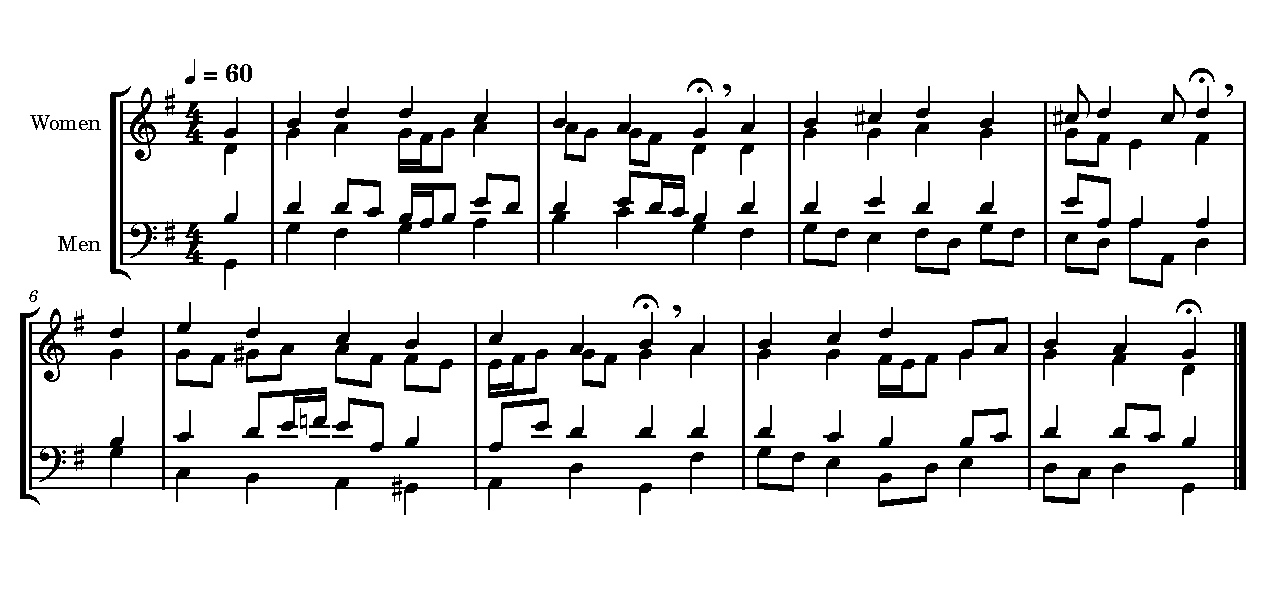
\includegraphics[width=0.75\textwidth, trim={0 30 0 30}, clip]{output26.pdf}\\ % {figures/alap-example.pdf}
       Das Beispiel zeigt einen unserer Ansicht nach gelungenen Choral im Stil von 
        Johann Sebastian Bach\\
        (Prompt: \texttt{Johann Sebastian Bach, Baroque, Choral})

  % \lilypondfile{output3.ly}
  
  % \vspace{1cm}
  
  % \begin{tikzpicture}[
  %   operation/.style={text opacity=0},
  %   every node/.style={circle,inner sep=5pt,font=\small},
  %   % xscale=0.325,yscale=0.6
  %   xscale=1.4,yscale=3
  %   ]
  %   % \node at (-3,0) {};
  %   \input{figures/alap_graph.tex}
  % \end{tikzpicture}
  % \begin{small}
  %   Selected phrases, in order of performance,
  %   from the ascending part of an \alap\ in \raga\ \multani,
  %   recorded by the sitarist Dharambir Singh.
  % \end{small}
  
  \vfill
  
  \begin{columns}[t]
    
    \begin{column}{0.25\textwidth}
      \begin{block}{1. Verteilung von Tonarten}
        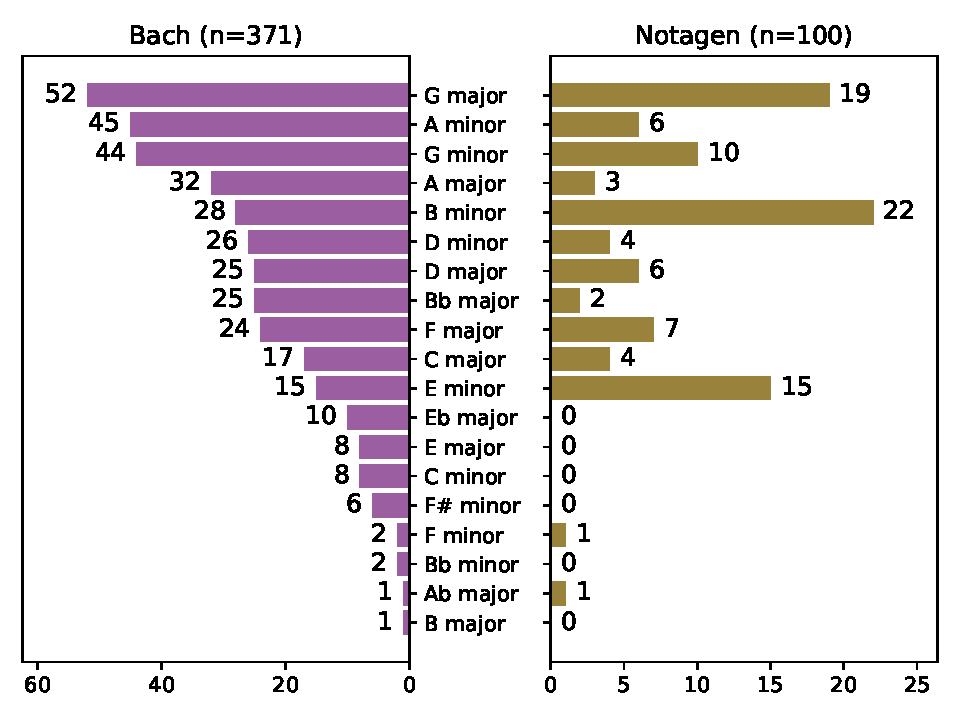
\includegraphics[width=\textwidth]{key_comparison.pdf}
        % Since both notes and intervals are elaborated,
        % melodies are represented as graphs with \alert{notes as nodes}
        % and \alert{intervals as edges}.
        % The elaboration operations then form an edge-replacement \alert{graph grammar}.
        %
        % Interval elaborations replace an edge with a new subgraph:
        % \[ (n_1 \to n_2) \longrightarrow (n_1 \to n' \to n_2) \]
        % Note elaboration also replace edges but consider only one of the nodes:
        % \[ (n_1 \to *) \longrightarrow (n_1 \to n' \to *) \]
        % Independent parts of the graph can be separated explicitly
        % by introducing an \alert{empty node}:
        % \[ (n_1 \to n_2) \longrightarrow (n_1 \to \varepsilon \to n_2) \]
        %
        % Another advantage of graphs is that they can capture more complex structures
        % such as \alert{polyphonic networks}.
      \end{block}
      \begin{block}{2. Verteilung von Taktarten}
        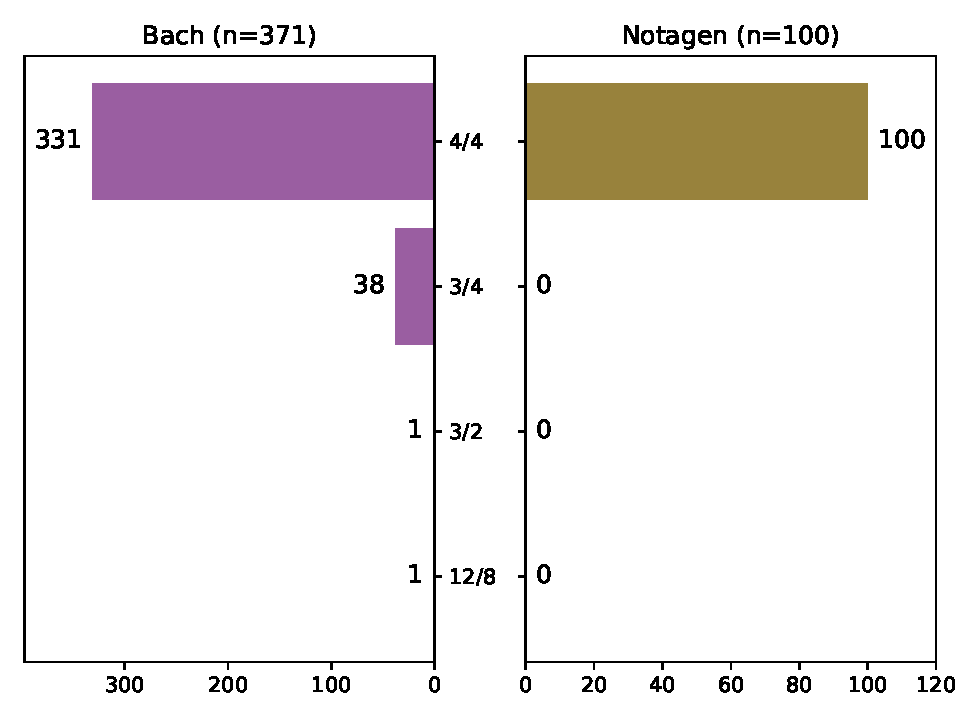
\includegraphics[width=\textwidth]{ts_comparison.pdf}
      \end{block}
    \end{column}

    \begin{column}{0.25\textwidth}
      \begin{block}{3. Akkordhäufigkeit}
        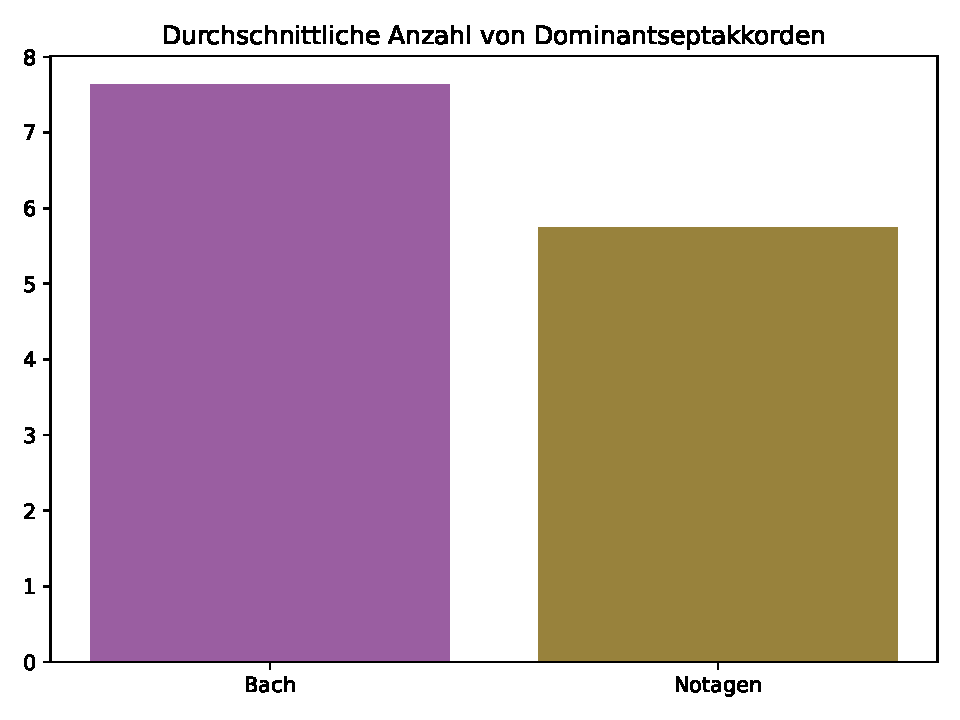
\includegraphics[width=\textwidth]{dominant_chords.pdf}
        % Since the graph of a monophonic melody is linear,
        % its derivation can be visualized by an \alert{outerplanar graph}
        % % \autocite{YustGeometryMelodicHarmonic2009},
        % where each polygon represents an edge replacement.
        %
        % \begin{tikzpicture}[
        %   operation/.append style={inner sep=3pt,font=\small},
        %   every edge/.append style={->,draw=black},
        %   scale=2.8
        %   ]
        %   \node[external node] (note0) at (0,0.0) {$\rtimes$};
        %   \node[note node] (note5) at (1,-1.5) {$7_\prime$};
        %   \node[note node] (note3) at (2,-1.0) {$1$};
        %   \node[epsilon node] (note4) at (3,-1.5) {$\varepsilon{}$};
        %   \node[note node] (note6) at (4,-2.0) {$\flat3$};
        %   \node[note node] (note7) at (5,-2.5) {$\flat2$};
        %   \node[note node] (note2) at (6,-0.5) {$1$};
        %   \node[external node] (note1) at (7,0.0) {$\ltimes$};
        %   \draw (note0) edge[external edge] node[operation,pos=0.8] {init} (note1);
        %   \draw (note0) edge[external edge] node[operation] {dup$\to{}$} (note2);
        %   \draw (note0) edge[external edge] node[operation,pos=0.6] {nb$\to{}$} (note3);
        %   \draw (note0) edge[external edge,surface edge] node[operation] {} (note5);
        %   \draw (note2) edge[external edge,surface edge] node[operation] {} (note1);
        %   \draw (note3) edge[] node[operation,pos=0.3] {split} (note2);
        %   \draw (note3) edge[epsilon edge,surface edge] node[operation] {} (note4);
        %   \draw (note4) edge[epsilon edge] node[operation,pos=0.4] {nb$\to{}$} (note2);
        %   \draw (note4) edge[epsilon edge,surface edge] node[operation] {} (note6);
        %   \draw (note5) edge[surface edge] node[operation] {} (note3);
        %   \draw (note6) edge[] node[operation,pos=0.4] {pass} (note2);
        %   \draw (note6) edge[surface edge] node[operation] {} (note7);
        %   \draw (note7) edge[surface edge] node[operation] {} (note2);
        % \end{tikzpicture}
        %
        % Indepencene is indicated by $\varepsilon$-nodes.
        % Adjacent edges are shown in light gray,
        % revealing the differences between note and interval elaborations.
        %
      \end{block}
      \begin{block}{Resultate}
        \begin{enumerate}
          \item Tonarten sind sehr unterschiedlich verteilt. 
          \item NotaGen `kennt' nur eine einzige Taktart (4/4).
          \item Dominantseptakkorde sind ähnlich verteilt, aber Bach benutzt mehr. Andere Akkordtypen müssen
            noch untersucht werden.
        \end{enumerate}
      \end{block}
    \end{column}
    
    \begin{column}{0.25\textwidth}

      \begin{block}{Link zum Experiment}
        \textbf{Könnt ihr den Unterschied hören?}
        % \begin{wrapfigure}{l}{\textwidth}
          \begin{center}
          \qrcode[height=0.5\textwidth]{https://fabianmoss.github.io/ai-chorales} \\
            \vspace{1em}
            \url{http://fabianmoss.github.io/ai-chorales}
          \end{center}
        % \end{wrapfigure}
                % The research presented on this poster is generously supported
        % by the Volkswagen Foundation and Claude Latour.
        % This project has received funding from the European Research Council (ERC)
        % under the European Union's Horizon 2020 research and innovation programme
        % under grant agreement No 760081 – PMSB.
        % We thank Dharambir Singh for the permission to use his recording of an
        % \alap\ in \raga\ \multani.

        % \begin{adjustbox}{valign=m}
        %   \includegraphics[width=0.5\textwidth]{../logos/epfl/logo_print.pdf}
        %   
\includegraphics[width=0.5\textwidth]{figures/soas.jpg}
        % \end{adjustbox}
      \end{block}
        \begin{block}{Referenzen}
          \printbibliography
        \end{block}
        % 
\includegraphics[width=\textwidth]{beamerthemeUniversityOfAmsterdam/logo/uva_logo_ENG.pdf}
        \begin{center}
          
\includegraphics[width=.75\linewidth]{unilogo_Vektor_CMYK.eps}
        \end{center}


        % \begin{adjustbox}{valign=m}
        % \includegraphics[width=0.5\textwidth,,trim=0 -2cm 0 0]{../logos/erc/flag.pdf}
        % \includegraphics[width=0.5\textwidth]{../logos/erc/erc.pdf}
        % \end{adjustbox}
    \end{column}
    
  \end{columns}

  \vfill
  
\end{frame} % End of the enclosing frame

\end{document}
% Local Variables:
% TeX-engine: luatex
% TeX-command-extra-options: "-shell-escape"
% End:
